%************************************************
\chapter*{Summary}
\chaptermark{Summary} %otherwise gets it wrong? Like for Introduction
\label{pt:summary}
In this thesis, we have studied how spatial inhomogeneities can prohibit a system's thermalization at least on short and intermediate timescales. We considered both closed quantum systems with long-range, power-law, interactions as well as periodically driven systems with nearest neighbor interactions and detailed for both scenarios how the spatial disorder leads to non-trivial, quasi-conserved, quantities. These effective conservation laws allow for making predictions about the systems recovering predictive power even in the absence of thermalization.

\FIXME{Expand first paragraph}

Additionally, by studying power-law interaction models subject to spatial disorder in Part \ref{pt:spatial-disorder}, we demonstrated that there is an emergent integrability similar to MBL. This featured appeared to be robust using numerical finite size scaling and the experimental data showed clear signatures of its consequences even in a critical case where $\alpha=d=3$. While the existence of MBL as a true thermodynamic phase is hotly debated, its core concept, i.e. the disorder-induced emergent integrability, proofed to be a very useful tool understand the behavior of real-world experiments. 

So while many systems, classical or quantum, thermalize quickly, there are exceptions to this rule when systems are subjected to disorder. These disordered systems evade a thermal description for long times or perhaps infinitely preventing a statistical understanding. For the systems studied here, the absence of thermalization was caused by effective conservation laws which could be exploited to gain insight into the systems' dynamics.
Speaking in terms of coffee: In a latte, the milk and coffee always intermix quickly. However if the milk is strongly
disordered, i.e. frothy, then it won't mix well into the coffee even if stirred  as is the case for a macchiato. At least in this regard, quantum systems are akin to coffee.

\begin{figure}[hbt]
	\centering
	\hfil
	\raisebox{-0.5\height}{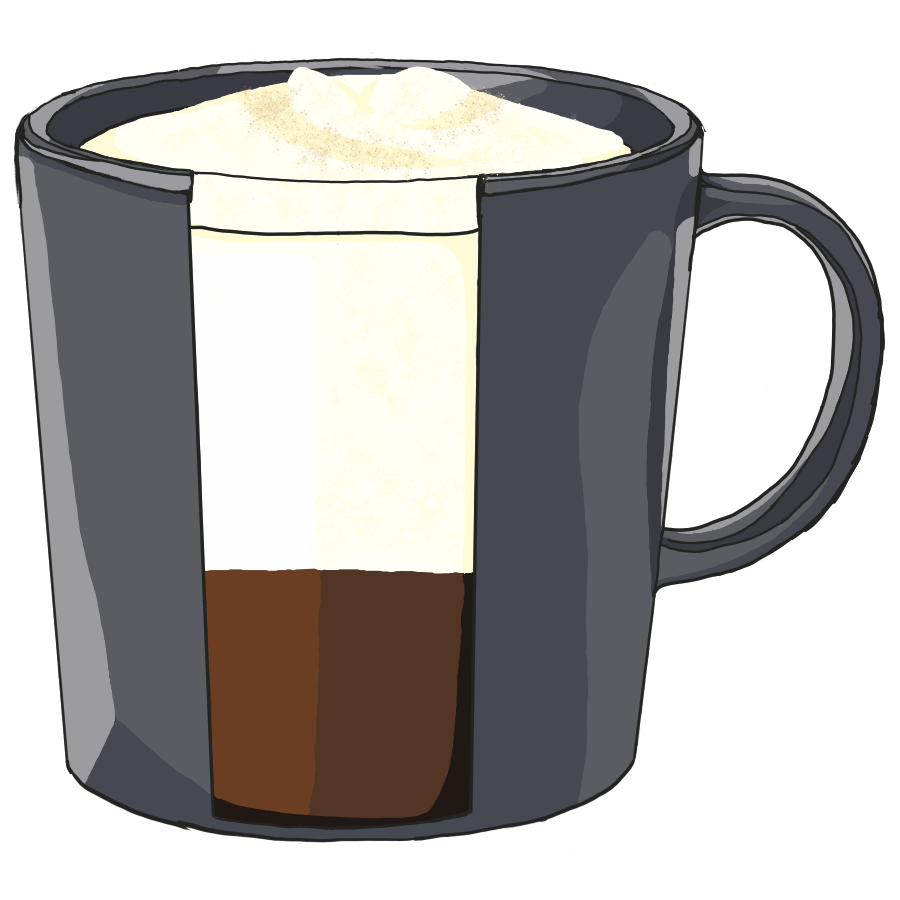
\includegraphics[width=0.3\textwidth]{gfx/intro/Kaffeetasse_Q1.png}}
	\hfil
	\raisebox{-0.5\height}{\scalebox{4}{$\longrightarrow$}}
	\hfil
	\raisebox{-0.5\height}{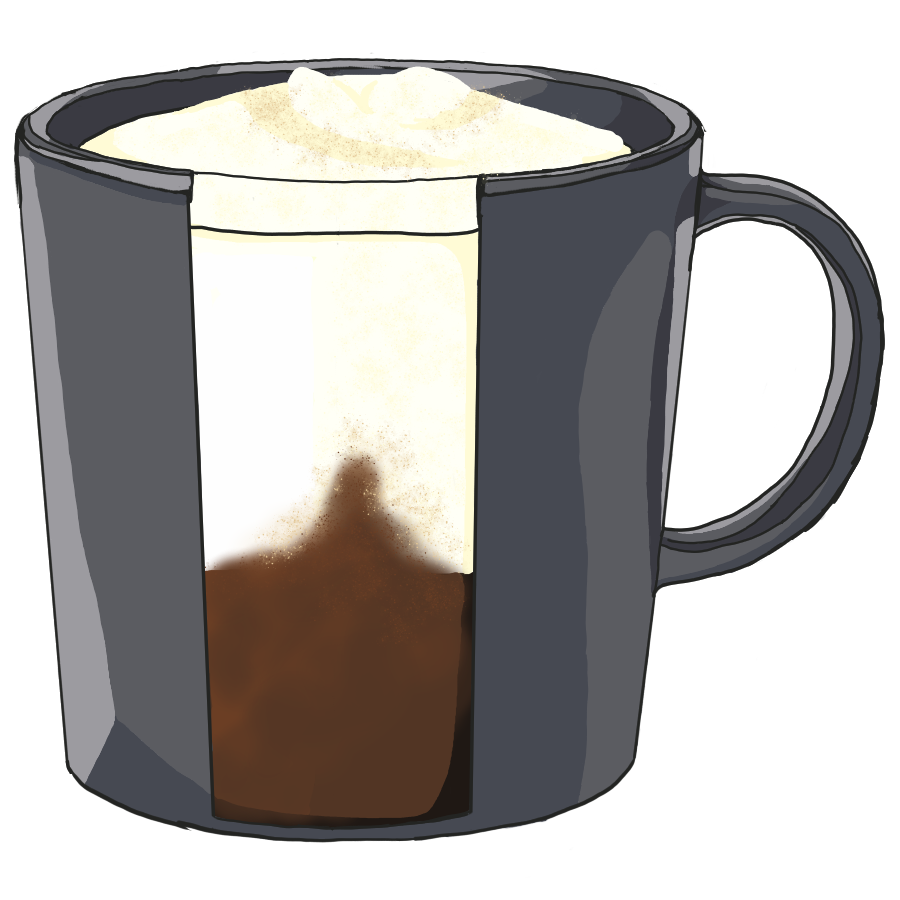
\includegraphics[width=0.3\textwidth]{gfx/intro/Kaffeetasse_Q2.png}}
	\hfil
	\caption{Classical localization of a macchiato.}
	\label{fig:localized-macciato}
\end{figure}

% i.e. behave like a cafe latte, where coffee and milk intermix quickly
%
%Two routes to non-thermalization (or to avoid thermalization at the usual short timescales) that both generate effectively conserved quantities in a subtle way.
%
%Bond-disordered systems are much more interesting than on-site disorder. More stable localization, but seems to not stabilize time crystalline signatures.

\FIXME{Should Summary exceed 1 page, check the page header of chapter is correct!}